Este tipo de características, que describen las propiedades de la señal en el dominio del tiempo, son muy simples;
y se computan directamente a partir de la señal digitalizada.

\subsection{Log-Attack Time}\label{subsec:log-attackTime}

El \textit{attack} de una señal se define como el espacio de tiempo, al inicio de esta, en que su intensidad va en ascenso.

El \textit{log-attack time} (LAT)~\cite{Gunasekaran11,Kim05,Manjunath02,Peters04} se calcula entonces como el logaritmo en base 10 de la duración del intervalo de tiempo transcurrido entre los momentos en que la señal se hace audible ($startAttack$) y en que alcanza su máxima intensidad ($stopAttack$):

\begin{equation}
    \label{eq:LAT}
    LAT = \log_{10}{(stopAttack - startAttack)}
\end{equation}

Los momentos $stopAttack$ y $startAttack$ suelen definirse como los puntos en que la potencia de la señal alcanza el 20\% y el 90\% de su máximo respectivamente.

\subsection{Audio Waveform}\label{subsec:audioWaveform}

Para computar esta característica se divide la señal en tramas no superpuestas ($M = N$), y se computan, por cada trama, los 2 valores siguientes:

\begin{itemize}
    \item Menor valor de amplitud de la señal presente en la trama.
    \item Mayor valor de amplitud de la señal presente en la trama.
\end{itemize}

El \textit{audio waveform} (AWF)~\cite{Kim05,Manjunath02} de la señal consistirá en un vector con los pares calculados, correspondientes a cada una de dichas tramas.

La extracción de esta característica puede ser vista como un modo de <<compresión>> de la señal.
Si se toma $N=1$ se obtendrá la propia señal, mientras que a medida que se seleccionen valores de $N$ más altos, el número de valores resultantes será cada vez menor, obteniéndose una representación reducida de la señal original.
El AWF puede representarse gráficamente como un conjunto de segmentos con extremos en los valores de la tupla correspondiente y desplazados en el tiempo relativo a su posición en la señal (figura~\ref{img:awf+ap}).

\subsection{Audio Power}\label{subsec:audioPower}

El \textit{audio power} (AP)~\cite{Kim05,Manjunath02} describe el comportamiento de la potencia de la señal en cada instante de tiempo.
Al igual que para la AWF, su cálculo requiere dividir la señal en tramas no superpuestas;
y se computa, para la trama $x[n]$ mediante la siguiente expresión:

\begin{equation}
    \label{eq:AP}
    AP = \frac{1}{N}\sum_{n=0}^{N-1}{|x[n]|^2}
\end{equation}

La representación gráfica del AP posibilita el análisis directo de la evolución de la amplitud de la señal en el transcurso del tiempo, lo que puede observarse en la figura~\ref{img:awf+ap}.

\begin{figure}[!h]
    \centering
    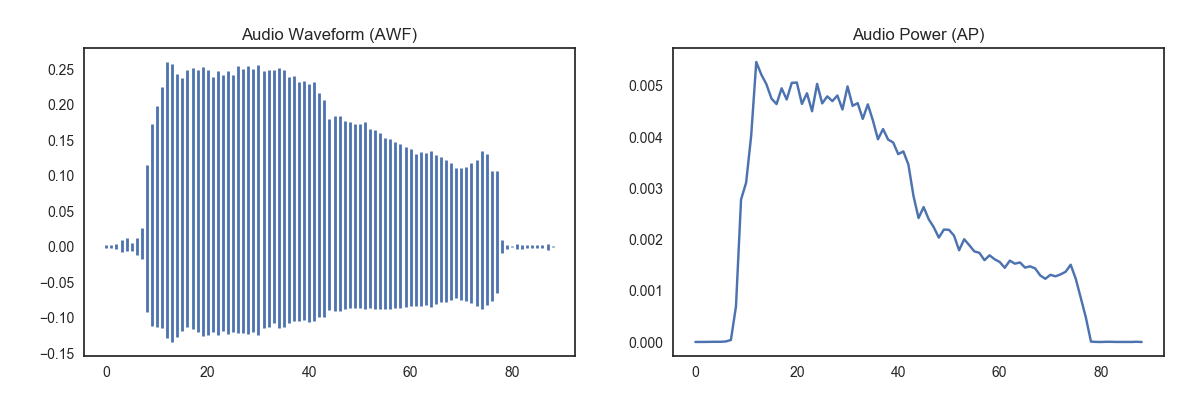
\includegraphics[width=\textwidth]{temporal-features.png}
    \caption{Dos características temporales básicas de una señal de audio: \textit{Audio Waveform} y \textit{Audio Power}, correspondientes a la señal de la figura~\ref{img:oscillogram}.}
    \label{img:awf+ap}
\end{figure}

\subsection{Temporal Centroid}\label{subsec:temporalCentroid}

El \textit{temporal centroid} (TC)~\cite{Kim05,Manjunath02,Peters04,Zamanian17} de la señal es el punto donde se localiza el centro de masas de su AP\@.
Se calcula mediante la siguiente expresión:

\begin{equation}
    \label{eq:TC}
    TC = \frac{\sum_{t=0}^{T-1}{AP_t \cdot t}}{\sum_{t=0}^{T-1}{AP_t}}
\end{equation}

\noindent
donde $T$ es la cantidad de tramas en que se descompuso la señal.

\subsection{Effective Duration}\label{subsec:effectiveDuration}

La \textit{effective duration} (ED)~\cite{Peters04} de una señal constituye la duración del intervalo de tiempo en que esta es perceptible;
el que generalmente se considera como el intervalo en que la amplitud de la señal permanece por encima del 40\% de su valor máximo.

\subsection{Auto-correlation}\label{subsec:auto-correlation}

La \textit{auto-correlation} (AC)~\cite{Gunasekaran11,Peters04} de la señal está dada por un vector de coeficientes que describen su distribución espectral en el dominio del tiempo.
El coeficiente $k$-ésimo se calcula mediante la expresión:

\begin{equation}
    \label{eq:AC}
    AC_k = \frac{1}{x[0]^2}\sum_{n=0}^{N-k-1}{x[n]\cdot x[n+k]}
\end{equation}

\subsection{Zero Crossing Rate}\label{subsec:zeroCrossingRate}

El \textit{zero crossing rate} (ZCR)~\cite{Fagerlund07,Gunasekaran11,Peters04} es una medida del número de veces que la amplitud de la señal cambia de signo.
Los sonidos periódicos tienden a tener un pequeño valor de ZCR, mientras que para los ruidos este valor suele ser alto.

Puede ser computado de forma global, o para cada trama de la señal, aplicando la siguiente expresión:

\begin{equation}
    \label{eq:ZCR}
    ZCR = \frac{1}{2}\sum_{n=1}^{N-1}{|\text{sign}(x[n]) - \text{sign}(x[n-1])|}
\end{equation}
